\section{ Object Recognition }
\subsection{Functional Requirements}
	\begin{flushleft}
		\begin{itemize}
			\item{\textbf{R3:}} FMDS will \textbf{detect objects} in the reserve
				\begin{itemize}
					\item{\textbf{R3.1}} FMDS will allow the ranger to see a list of \textbf{objects} and their \textbf{locations}.
						\begin{itemize}
							\item If an object is selected, the ranger will be pointed towards the detected object. Individual estimated threat levels will be displayed per object along with the object's classification.
						\end{itemize} 
					\item{\textbf{R3.2}} FMDS will draw a rectangle around the objects that it detects.
						\begin{itemize}
							\item Rectangles will be coloured and a label will be placed above the rectangle with the object's classification.
						\end{itemize} 
					\item{\textbf{R3.2}} FMDS will notify the ranger of the objects that it detects.
						\begin{itemize}
							\item The ranger will be notified of newly detected objects, their estimated threat level, classification and relative direction from the ranger.
						\end{itemize} 
				\end{itemize}
		\end{itemize}
	\end{flushleft}

\subsection{Use Case Diagram}
\begin{flushleft}
	\begin{figure}[h!]
		\centering
		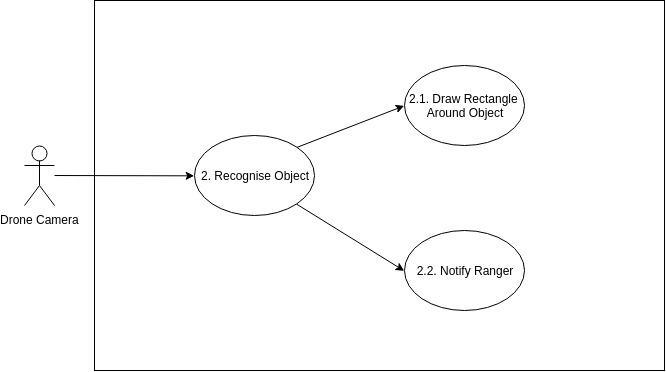
\includegraphics[scale=0.5]{./assets/images/object-recognition-ucd.jpg}
		\label{fig: object-recognition-ucd }
		\caption{Object Recognition Use Case Diagram}
	\end{figure}

\end{flushleft}

